\section{Systemaufbau}
\begin{center}
	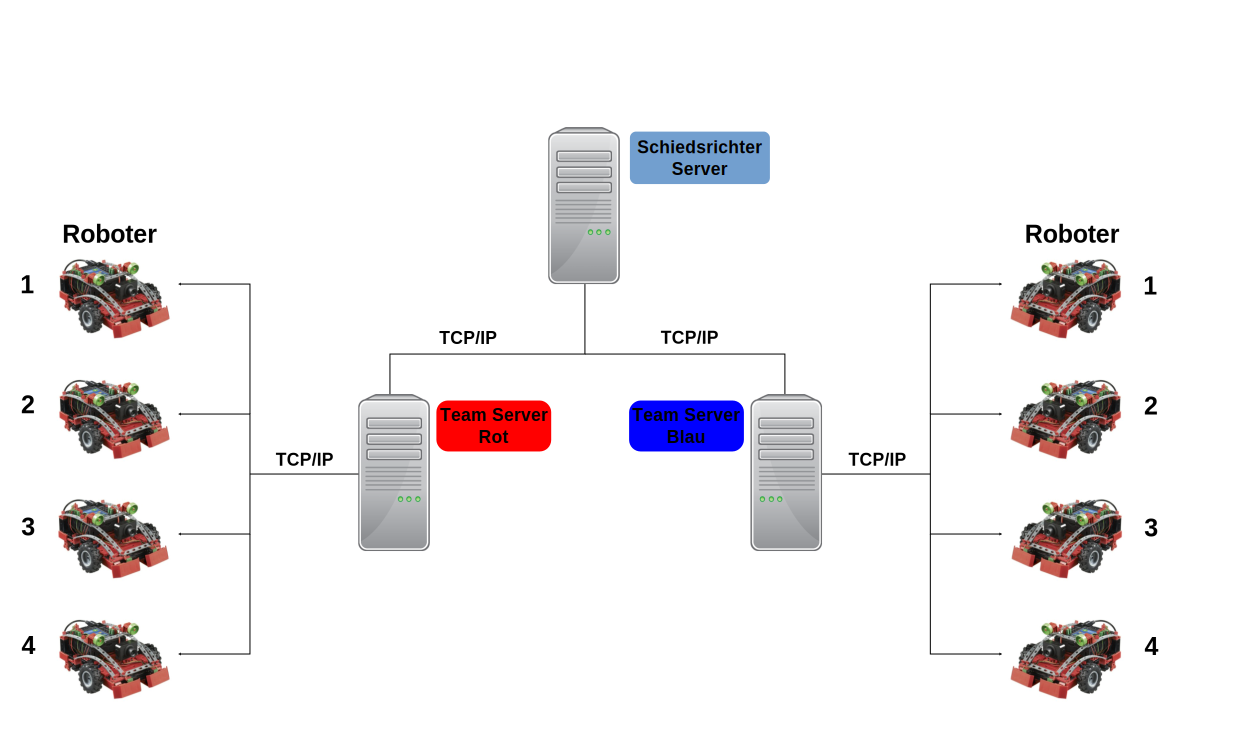
\includegraphics[width=1\textwidth]{Bilder/Systemaufbau.pdf}
	\captionof{figure}{Systemaufbau}
\end{center}
Der Systemaufbau des Projekts stellt sich wie folgt dar:
\\\\
Ein zentraler Schiedsrichter-Server überwacht das Spielfeld der Roboter mithilfe einer Kamera. Anhand des Kamerabildes werden Positionsdaten der Roboter bestimmt. Des weiteren überwacht der Server den Status der Roboter, d.h. es wird überprüft ob diese gefangen wurden.  

Die Positionsdaten werden mittels einer WLAN-Verbindung und des TCP/IP-Protokolls an die jeweiligen Team-Server gesendet. 
Diese werten die Daten aus und ermitteln die Fahrtrichtungen für jeden Roboter eines Teams. Die Befehle werden wieder mithilfe einer TCP/IP-Verbindung an die Roboter übermittelt.